\documentclass[conference]{IEEEtran}
\IEEEoverridecommandlockouts

% ===== Packages =====
\usepackage[utf8]{inputenc}
\usepackage[T5,T1]{fontenc}
\usepackage{cite}
\usepackage{amsmath,amssymb,amsfonts}
\usepackage{algorithmic}
\usepackage{graphicx}
\usepackage{textcomp}
\usepackage{xcolor}
\usepackage{booktabs}
\usepackage{multirow}
\usepackage{array}
\usepackage{url}
\usepackage{hyperref}
\usepackage{balance}
\usepackage{tikz}
\usetikzlibrary{arrows.meta,positioning,fit,shapes.geometric}

\def\BibTeX{{\rm B\kern-.05em{\sc i\kern-.025em b}\kern-.08em
    T\kern-.1667em\lower.7ex\hbox{E}\kern-.125emX}}

\begin{document}
\pagestyle{plain}
\pagenumbering{arabic}

\title{Abstractive Text Summarization Using a Transformer Implemented from Scratch and a Fine-tuned Pre-trained Language Model}

\author{
\IEEEauthorblockN{Mai Kha Anh, Nguyen Ngoc Dinh, Nguyen Thac Cuong, Nguyen Phi Anh}
\IEEEauthorblockA{\textit{Faculty of Information Technology} \\
\textit{University of Engineering and Technology, VNU}\\
Hanoi, Vietnam \\
Email: \{23020006, 23020009, 23030018, 23020021\}@vnu.edu.vn}
}

\maketitle
\thispagestyle{plain}

\begin{abstract}
Abstractive text summarization aims to generate a concise summary that preserves the main information of a long input document. In this project, we investigate two approaches for Vietnamese abstractive summarization. The first is an 11.47M-parameter sequence-to-sequence Transformer implemented from scratch in PyTorch. The second fully fine-tunes the 227.72M-parameter Vietnamese pre-trained encoder-decoder model ViT5-base. We additionally study parameter-efficient LoRA fine-tuning, BARTpho, a summarization warm-start checkpoint, Qwen3-1.7B with LoRA, prompt design, context length, and decoding configurations. On the full test set, the scratch Transformer obtains ROUGE-1/2/L scores of 0.5747/0.2038/0.3045, whereas ViT5-base obtains 0.7422/0.4675/0.4889. These results demonstrate the large benefit of Vietnamese-specific pre-training while also showing the efficiency--quality trade-off of LoRA and the importance of context length for causal language models.
\end{abstract}

\begin{IEEEkeywords}
abstractive summarization, Transformer, sequence-to-sequence learning, pre-trained language model, ROUGE, Vietnamese NLP
\end{IEEEkeywords}

% =========================================================
\section{Introduction}
Text summarization is an important task in natural language processing (NLP), where the goal is to condense a long document into a shorter version while preserving the most important information. Summarization systems are useful in news aggregation, document search, information retrieval, education, and digital assistants. Compared with extractive summarization, which selects important sentences directly from the source document, abstractive summarization generates new sentences and can produce more natural and concise summaries.

In this project, we focus on abstractive text summarization. Given an input document $X = (x_1, x_2, \ldots, x_m)$, the system is required to generate a shorter target summary $Y = (y_1, y_2, \ldots, y_n)$, where $n < m$ in most cases. The generated summary should be fluent, concise, and faithful to the original content.

The project requires two parallel approaches. The first approach is to build and train a Transformer model from scratch. This means that the core components, including multi-head attention, positional encoding, encoder, decoder, and feed-forward network, must be implemented manually using basic PyTorch modules, without directly using high-level modules such as \texttt{nn.Transformer}. The second approach is to fine-tune a pre-trained language model with fewer than 3 billion parameters.

The main contributions of our work are as follows:
\begin{itemize}
    \item We implement a complete encoder-decoder Transformer architecture from scratch for abstractive summarization.
    \item We build the full data pipeline, including text cleaning, JSONL conversion, subword tokenizer training, tokenization cache creation, and mini-batch masking.
    \item We implement practical training and decoding improvements such as Pre-LN blocks, label smoothing, shared embeddings, weight tying, warmup scheduling, gradient clipping, beam search, length penalty, and no-repeat n-gram blocking.
    \item We evaluate the trained Transformer using ROUGE metrics, repetition statistics, validation decoding comparison, and the public test set.
    \item We fully fine-tune ViT5-base and compare it with ViT5 LoRA, BARTpho, a ViT5 summarization warm start, and LoRA-adapted causal language models under the assignment's 3-billion-parameter limit.
    \item We conduct controlled Qwen3 ablations on prompt design, LoRA rank, context length, and training-set size using validation subsets.
\end{itemize}

% =========================================================
\section{Related Work}
Early neural summarization systems were commonly based on recurrent neural networks and sequence-to-sequence architectures with attention mechanisms. These models encode the input sequence into hidden representations and decode the summary token by token. However, recurrent models are difficult to parallelize and may struggle with long-range dependencies.

The Transformer architecture introduced by Vaswani et al. replaced recurrence with self-attention, allowing the model to capture dependencies between arbitrary positions in a sequence more efficiently. The original Transformer consists of an encoder stack and a decoder stack, where each layer contains attention mechanisms, feed-forward networks, residual connections, and layer normalization. Our implementation keeps this encoder-decoder structure and implements the core components manually, while using a few explicit training-oriented modifications described in the methodology.

Pre-trained language models further improved many NLP tasks by learning general-purpose representations from large-scale corpora. Models such as BART \cite{lewis2020bart}, T5, mBART, and PEGASUS \cite{zhang2020pegasus} are widely used for summarization because they are pre-trained with denoising or sequence-to-sequence objectives. Fine-tuning these models on a downstream summarization dataset often provides stronger results than training a model from scratch, especially when the task dataset is limited.

For Vietnamese generation, ViT5 adapts the T5 text-to-text encoder-decoder framework to large Vietnamese corpora and reports strong abstractive-summarization performance \cite{phan2022vit5}. BARTpho is a monolingual Vietnamese sequence-to-sequence model based on the BART denoising objective \cite{tran2022bartpho}. We use ViT5-base as the primary pre-trained model because its architecture directly matches conditional summary generation and its Vietnamese-specific pre-training is well aligned with the dataset.

Parameter-efficient fine-tuning methods reduce the cost of adapting large pre-trained models. LoRA freezes the original weights and learns low-rank update matrices, greatly reducing the number of trainable parameters \cite{hu2022lora}. We apply LoRA to both ViT5 and causal language models. Qwen3 is included as an additional multilingual causal-LM comparison because the 1.7B dense model satisfies the assignment's parameter limit and supports instruction-based generation \cite{yang2025qwen3}.

% =========================================================
\section{Methodology}

\subsection{Task Formulation}
The task is formulated as conditional sequence generation. Given a source document $X$, the model estimates the probability of a target summary $Y$ as:
\begin{equation}
P(Y|X) = \prod_{t=1}^{n} P(y_t | y_{<t}, X).
\end{equation}
During training, teacher forcing is used, where the decoder receives the previous ground-truth tokens. During inference, the summary is generated autoregressively until the end-of-sequence token is produced or the maximum decoding length is reached.

\subsection{Tokenization and Data Processing}
We use a SentencePiece BPE subword tokenizer trained on the provided training corpus. The preprocessing pipeline first inspects the parquet files, normalizes each example into a source--target pair, removes invalid or extremely short samples, and stores the cleaned data as JSONL files. The tokenizer then converts input documents and target summaries into sequences of token IDs. Special tokens include \texttt{<PAD>}, \texttt{<UNK>}, \texttt{<BOS>}, and \texttt{<EOS>}. Long documents are truncated to a maximum source length, and summaries are truncated to a maximum target length. Tokenized examples are cached as pickle files to avoid repeating the preprocessing step during training.

\begin{itemize}
    \item Tokenizer type: SentencePiece BPE
    \item Vocabulary size: 16000
    \item Maximum source length: 512 tokens
    \item Maximum target length: 128 tokens
    \item Filtering rules: source length from 30 to 900 words, target length from 3 to 180 words, and target/source length ratio at most 0.9
    \item Training samples: 10775
    \item Validation samples: 1349
    \item Test samples: 1344
\end{itemize}

\subsection{Transformer from Scratch}
Our first model is an encoder-decoder Transformer implemented from scratch. The model follows the main encoder-decoder design of the Transformer in \cite{vaswani2017attention}: token embeddings, sinusoidal positional encoding, multi-head attention, feed-forward networks, residual connections, encoder and decoder stacks, and a final vocabulary projection. For training stability and summarization quality, the implemented model intentionally uses Pre-LN blocks, GELU activation, shared source-target embeddings, output weight tying, label smoothing, warmup scheduling, beam search, length penalty, and no-repeat n-gram blocking. These changes are reported as implementation improvements rather than as exact components of the original paper.

\begin{figure*}[htbp]
\centering
\resizebox{0.95\textwidth}{!}{%
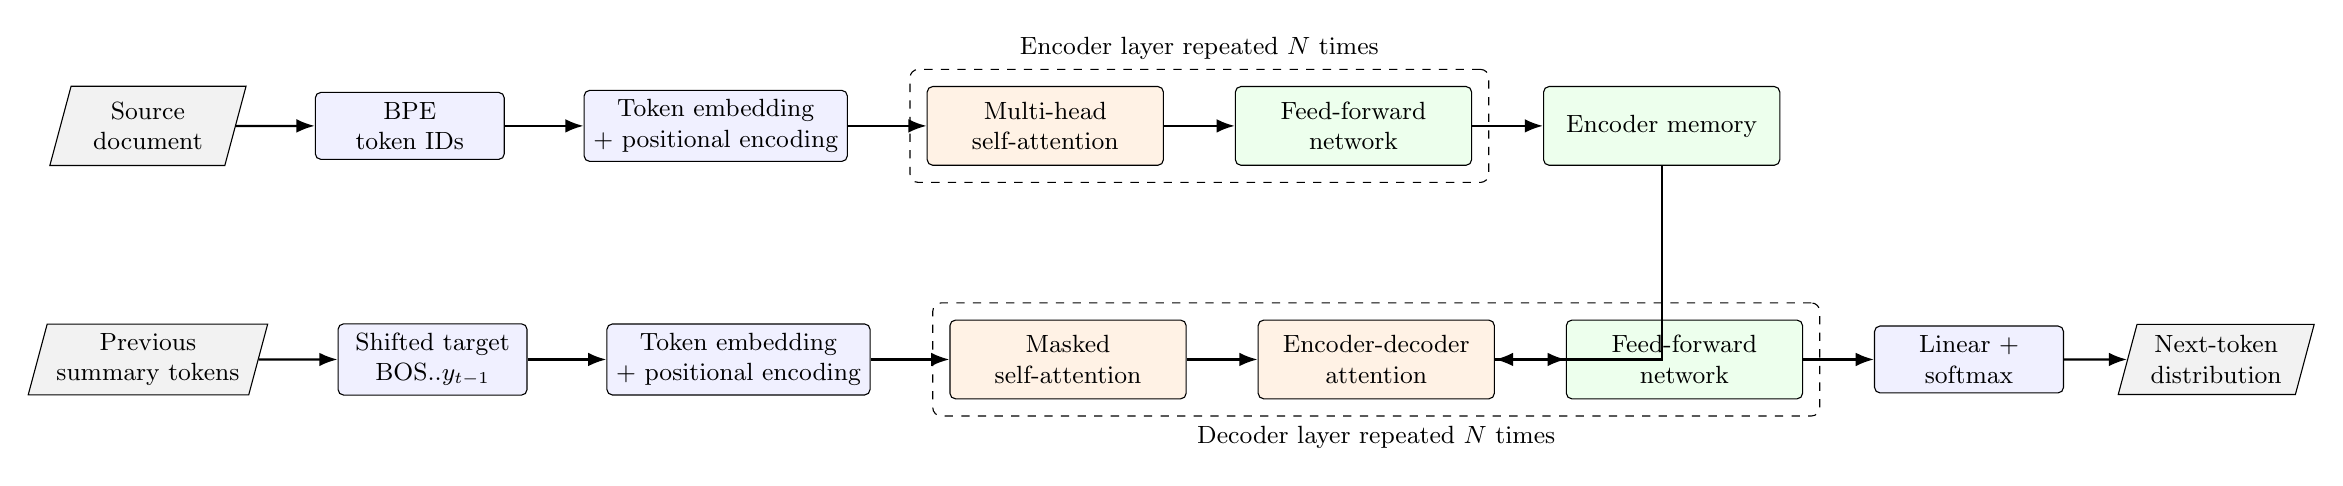
\begin{tikzpicture}[
    font=\small,
    box/.style={draw, rounded corners=2pt, align=center, minimum width=2.4cm, minimum height=0.85cm, fill=blue!6},
    block/.style={draw, rounded corners=2pt, align=center, minimum width=3.0cm, minimum height=1.0cm, fill=green!7},
    attn/.style={draw, rounded corners=2pt, align=center, minimum width=3.0cm, minimum height=1.0cm, fill=orange!10},
    io/.style={draw, trapezium, trapezium left angle=75, trapezium right angle=105, align=center, minimum width=2.5cm, minimum height=0.8cm, fill=gray!10},
    arrow/.style={-Latex, thick}
]
\node[io] (src) {Source\\document};
\node[box, right=1.0cm of src] (src_tok) {BPE\\token IDs};
\node[box, right=1.0cm of src_tok] (src_emb) {Token embedding\\+ positional encoding};
\node[attn, right=1.0cm of src_emb] (enc_attn) {Multi-head\\self-attention};
\node[block, right=0.9cm of enc_attn] (enc_ffn) {Feed-forward\\network};
\node[block, right=0.9cm of enc_ffn] (memory) {Encoder memory};

\node[io, below=2.0cm of src] (tgt) {Previous\\summary tokens};
\node[box, right=1.0cm of tgt] (tgt_tok) {Shifted target\\BOS..$y_{t-1}$};
\node[box, right=1.0cm of tgt_tok] (tgt_emb) {Token embedding\\+ positional encoding};
\node[attn, right=1.0cm of tgt_emb] (dec_self) {Masked\\self-attention};
\node[attn, right=0.9cm of dec_self] (cross) {Encoder-decoder\\attention};
\node[block, right=0.9cm of cross] (dec_ffn) {Feed-forward\\network};
\node[box, right=0.9cm of dec_ffn] (softmax) {Linear +\\softmax};
\node[io, right=0.8cm of softmax] (out) {Next-token\\distribution};

\draw[arrow] (src) -- (src_tok);
\draw[arrow] (src_tok) -- (src_emb);
\draw[arrow] (src_emb) -- (enc_attn);
\draw[arrow] (enc_attn) -- (enc_ffn);
\draw[arrow] (enc_ffn) -- (memory);
\draw[arrow] (tgt) -- (tgt_tok);
\draw[arrow] (tgt_tok) -- (tgt_emb);
\draw[arrow] (tgt_emb) -- (dec_self);
\draw[arrow] (dec_self) -- (cross);
\draw[arrow] (cross) -- (dec_ffn);
\draw[arrow] (dec_ffn) -- (softmax);
\draw[arrow] (softmax) -- (out);
\draw[arrow] (memory) |- (cross);

\node[draw, dashed, rounded corners=3pt, fit=(enc_attn)(enc_ffn), inner sep=6pt, label=above:{Encoder layer repeated $N$ times}] {};
\node[draw, dashed, rounded corners=3pt, fit=(dec_self)(cross)(dec_ffn), inner sep=6pt, label=below:{Decoder layer repeated $N$ times}] {};
\end{tikzpicture}
}
\caption{Architecture of the from-scratch encoder-decoder Transformer used for abstractive summarization. Padding masks are used in the encoder and cross-attention, while a causal mask is used in decoder self-attention.}
\label{fig:architecture}
\end{figure*}

\subsubsection{Embedding and Positional Encoding}
Since the Transformer has no recurrence or convolution, positional information must be injected into token embeddings. For a position $pos$ and dimension $i$, the sinusoidal positional encoding is defined as:
\begin{equation}
PE_{(pos, 2i)} = \sin\left(\frac{pos}{10000^{2i/d_{model}}}\right),
\end{equation}
\begin{equation}
PE_{(pos, 2i+1)} = \cos\left(\frac{pos}{10000^{2i/d_{model}}}\right).
\end{equation}
The input representation is obtained by adding token embeddings and positional encodings. In our implementation, source and target embeddings are shared because both sequences are Vietnamese text, and the output projection is tied with the target embedding matrix to reduce parameters and improve generalization.

\subsubsection{Scaled Dot-Product Attention}
The core operation of the Transformer is scaled dot-product attention:
\begin{equation}
\mathrm{Attention}(Q,K,V) = \mathrm{softmax}\left(\frac{QK^T}{\sqrt{d_k}}\right)V,
\end{equation}
where $Q$, $K$, and $V$ are query, key, and value matrices, and $d_k$ is the dimension of the key vectors. Padding masks are applied to ignore padded tokens, while causal masks are applied in the decoder to prevent the model from attending to future target tokens.

\subsubsection{Multi-Head Attention}
Instead of computing a single attention function, multi-head attention projects the input into multiple representation subspaces:
\begin{equation}
\mathrm{head}_i = \mathrm{Attention}(QW_i^Q, KW_i^K, VW_i^V),
\end{equation}
\begin{equation}
\mathrm{MultiHead}(Q,K,V) = \mathrm{Concat}(\mathrm{head}_1, \ldots, \mathrm{head}_h)W^O.
\end{equation}
This allows the model to attend to different semantic and positional relationships simultaneously.

\subsubsection{Position-wise Feed-Forward Network}
Each encoder and decoder layer includes a position-wise feed-forward network:
\begin{equation}
\mathrm{FFN}(x) = \mathrm{GELU}(xW_1 + b_1)W_2 + b_2.
\end{equation}
The same feed-forward network is applied independently to each position. The original Transformer uses ReLU, while our implementation uses GELU as a small practical modification.

\subsubsection{Encoder Layer}
Each encoder layer contains a multi-head self-attention sublayer followed by a feed-forward sublayer. Our implementation uses the Pre-LN variant, where layer normalization is applied before each sublayer to make optimization more stable:
\begin{equation}
\tilde{x} = x + \mathrm{SelfAttention}(\mathrm{LayerNorm}(x)),
\end{equation}
\begin{equation}
z = \tilde{x} + \mathrm{FFN}(\mathrm{LayerNorm}(\tilde{x})).
\end{equation}

\subsubsection{Decoder Layer}
Each decoder layer contains three sublayers: masked self-attention, encoder-decoder attention, and a feed-forward network. Masked self-attention ensures that token $y_t$ only depends on previous target tokens. Encoder-decoder attention allows the decoder to attend to the encoded source document. The decoder also follows the Pre-LN structure with residual connections and dropout around each sublayer.

\subsubsection{Training Objective}
The model is trained using cross-entropy loss over the target sequence. During training, the target sequence is shifted: the decoder input is \texttt{BOS..token\_n-1}, and the labels are \texttt{token\_1..EOS}. Padding tokens are ignored when computing the loss, and label smoothing is used to reduce overconfidence:
\begin{equation}
\mathcal{L} = -\sum_{t=1}^{n} \log P(y_t | y_{<t}, X).
\end{equation}
The optimizer is AdamW with Transformer-style linear warmup followed by inverse-square-root decay. Gradients are clipped to avoid unstable updates on long documents.

\subsection{Pre-trained Model Fine-tuning}
The primary model for the second approach is \texttt{VietAI/vit5-base}, a Vietnamese text-to-text Transformer based on the T5 encoder-decoder architecture \cite{raffel2020t5,phan2022vit5}. The loaded checkpoint contains 227,720,448 parameters, which is far below the assignment limit of 3 billion parameters. ViT5 is selected because it is pre-trained specifically for Vietnamese, directly supports sequence-to-sequence generation, and has previously demonstrated strong Vietnamese summarization performance.

Each article is prefixed with \texttt{summarize:} and tokenized to at most 768 source tokens; the target summary is limited to 160 tokens. We fully fine-tune all ViT5 parameters with the teacher-forced sequence-to-sequence cross-entropy objective. Training uses AdamW, a peak learning rate of $3\times10^{-5}$, cosine decay, a 0.06 warmup ratio, weight decay of 0.01, label smoothing of 0.1, dropout of 0.1, gradient checkpointing, and three epochs. Checkpoints are selected by validation ROUGE-L. The final generation configuration uses beam size 4, length penalty 1.0, repetition penalty 1.05, and no-repeat 3-gram blocking.

We also evaluate parameter-efficient LoRA fine-tuning. For an original weight matrix $W$, LoRA freezes $W$ and learns a low-rank update:
\begin{equation}
W' = W + \frac{\alpha}{r}BA,
\end{equation}
where $A$ and $B$ are trainable matrices and $r$ is the rank. ViT5 LoRA uses rank 16, $\alpha=32$, and dropout 0.05 on the query and value projections. It trains only 1,769,472 parameters, or 0.777\% of the 227.72M-parameter model.

As an additional improvement branch, we adapt Qwen3-1.7B with LoRA. The input contains a Vietnamese summarization instruction followed by the article; labels for the instruction and article tokens are masked with $-100$, so the loss is computed only on summary tokens. Controlled experiments compare a basic prompt with a strict faithfulness prompt, LoRA ranks 8 and 16, source contexts of 768 and 1024 tokens, and different training-set sizes. This causal-LM branch is reported separately because its validation and test experiments use subsets for computational efficiency.

BARTpho-syllable and \texttt{VietAI/vit5-base-vietnews-summarization} are evaluated as additional sequence-to-sequence comparisons. Because the latter checkpoint was already adapted to Vietnamese news summarization, it is treated as a warm-start experiment rather than the primary baseline.

\subsection{Method Improvements}
To improve the scratch Transformer system, we implement several practical techniques.

The following techniques are implemented in the current codebase for the scratch Transformer:
\begin{itemize}
    \item \textbf{Beam search decoding}: considers multiple candidate summaries during inference instead of selecting only the most probable token at each step.
    \item \textbf{Dropout}: reduces overfitting in attention, embedding, and feed-forward layers.
    \item \textbf{Learning-rate warmup}: stabilizes early Transformer training, followed by inverse-square-root decay.
    \item \textbf{Label smoothing}: prevents the model from becoming overconfident.
    \item \textbf{Shared embeddings and weight tying}: reduce the number of trainable parameters.
    \item \textbf{Gradient clipping}: limits gradient spikes during training.
    \item \textbf{No-repeat n-gram blocking}: discourages repetitive generated summaries.
\end{itemize}

For the pre-trained approach, the main improvements and comparisons are:
\begin{itemize}
    \item \textbf{Full fine-tuning versus LoRA}: measures the quality--efficiency trade-off when only 0.777\% of ViT5 parameters are trainable.
    \item \textbf{Vietnamese model comparison}: compares ViT5-base with BARTpho-syllable and a ViT5 checkpoint already adapted to Vietnamese news summarization.
    \item \textbf{Causal-LM prompt and context ablations}: tests strict instructions, LoRA rank, longer context, and additional training data for Qwen3-1.7B.
    \item \textbf{Decode sensitivity analysis}: compares beam sizes, length penalties, and output-length constraints for the same ViT5 checkpoint.
\end{itemize}

% =========================================================
\section{Experiments and Results}

\subsection{Dataset}
The dataset is provided by the course instructor. Each example contains two fields: \texttt{article}, which stores the source document, and \texttt{summary}, which stores the reference summary. We perform descriptive analysis only on the training and validation splits. The held-out test split follows the same two-field structure and is used only once for final evaluation; no test examples or test statistics are used for training, model selection, or dataset analysis.

\begin{table}[htbp]
\centering
\caption{Train/validation length statistics in Unicode word units.}
\label{tab:dataset}
\resizebox{\columnwidth}{!}{%
\begin{tabular}{lrrrr}
\toprule
Split & Samples & Article mean/med./P90 & Summary mean/med./P90 & Comp. \\
\midrule
Train & 10775 & 463.0/449/620 & 103.8/101/135 & 0.232 \\
Validation & 1349 & 471.2/455/632 & 103.3/101/135 & 0.227 \\
\bottomrule
\end{tabular}
}
\end{table}

The two analyzed splits have closely matched distributions. A source article contains about 463--471 words on average, while a reference summary contains about 103 words and retains approximately 23\% of the source length. The 90th-percentile article lengths are 620 and 632 words for train and validation, respectively, indicating that many examples require processing substantially more than the opening paragraph.

\begin{table}[htbp]
\centering
\caption{Article--summary characteristics on train and validation.}
\label{tab:dataset_overlap}
\resizebox{\columnwidth}{!}{%
\begin{tabular}{lrr}
\toprule
Metric & Train & Validation \\
\midrule
Summary unigram overlap recall & 0.9226 & 0.9251 \\
Summary bigram overlap recall & 0.6814 & 0.6899 \\
Novel summary unigram ratio & 0.0643 & 0.0622 \\
Novel summary bigram ratio & 0.3106 & 0.3023 \\
Summary coverage by first 25\% of article & 0.5034 & 0.5131 \\
Summary coverage by first 50\% of article & 0.7292 & 0.7351 \\
References longer than 128 words & 15.53\% & 15.05\% \\
References longer than 160 words & 0.29\% & 0.30\% \\
Reference-number support in article & 97.28\% & 96.93\% \\
\bottomrule
\end{tabular}
}
\end{table}

The references are abstractive but highly grounded in the source. On validation, 92.51\% of reference unigrams and 68.99\% of reference bigrams occur in the corresponding article, while 30.23\% of summary bigrams are novel. Thus, a successful system must both preserve source phrases and reorganize them into a concise output. Only 51.31\% of summary unigrams are covered by the first quarter of the article, increasing to 73.51\% for the first half; later article content therefore remains important. Numerical faithfulness is also central because 96.93\% of numbers appearing in validation summaries are supported by their source articles.

The train/validation similarity supports stable model selection on validation. The final validation and held-out test ROUGE scores are also close for both the scratch Transformer and ViT5, suggesting no major distribution shift under the instructor-provided split construction without requiring any descriptive analysis of the test content.
\subsection{Experimental Setup}
The implementation is based on PyTorch and Hugging Face Transformers. Experiments are run on a Kaggle instance with two Tesla T4 GPUs, each with 15\,GB of memory. The scratch Transformer is trained from random initialization. ViT5 and the other pre-trained models are adapted from public checkpoints, while all reported models remain below 3 billion parameters. Unless a subset is explicitly stated, validation results use all 1,349 validation examples and test results use all 1,344 test examples.

\begin{table}[htbp]
\centering
\caption{Hyperparameters for the Transformer from scratch.}
\label{tab:hparams_scratch}
\begin{tabular}{lr}
\toprule
Hyperparameter & Value \\
\midrule
Vocabulary size & 16000 \\
Number of encoder layers & 4 \\
Number of decoder layers & 4 \\
Model dimension $d_{model}$ & 256 \\
Feed-forward dimension $d_{ff}$ & 1024 \\
Number of attention heads & 8 \\
Dropout & 0.1 \\
Batch size & 4 \\
Optimizer & AdamW \\
Learning rate & $3 \times 10^{-4}$ \\
Epochs & 10 \\
Max source length & 512 \\
Max target length & 128 \\
Decoding method & Beam search, beam size 4 \\
Trainable parameters & 11469824 \\
Hardware & Kaggle GPU \\
\bottomrule
\end{tabular}
\end{table}

\begin{table}[htbp]
\centering
\caption{Hyperparameters for pre-trained model fine-tuning.}
\label{tab:hparams_pretrained}
\resizebox{\columnwidth}{!}{%
\begin{tabular}{lr}
\toprule
Hyperparameter & Value \\
\midrule
Pre-trained model & VietAI/vit5-base \\
Number of parameters & 227,720,448 \\
Batch size & 4/GPU, effective batch 16 \\
Learning rate & $3 \times 10^{-5}$ \\
Epochs & 3 \\
Max source length & 768 \\
Max target length & 160 \\
Decoding method & Beam 4, length penalty 1.0 \\
Hardware & 2$\times$ Tesla T4, FP16 \\
\bottomrule
\end{tabular}
}
\end{table}

\subsection{Evaluation Metrics}
We evaluate the generated summaries using ROUGE metrics \cite{lin2004rouge}, which are required for the assignment. ROUGE-1 measures unigram overlap, ROUGE-2 measures bigram overlap, and ROUGE-L measures the longest common subsequence between the generated summary and the reference summary. We report F1 scores for all ROUGE metrics. The pre-trained-model evaluation code emits ROUGE on a 0--100 scale; all report tables divide those values by 100 to use the same 0--1 scale as the scratch-Transformer results. In addition, we track repeated 3-gram ratio for the scratch system and generated token length for the pre-trained systems.

\subsection{Quantitative Results}
Table~\ref{tab:main_results} compares the two required approaches on the full validation set. Full ViT5 fine-tuning improves ROUGE-L from 0.3053 to 0.4924. ViT5 LoRA is more parameter-efficient but trails full fine-tuning by 0.0190 ROUGE-L.

\begin{table}[htbp]
\centering
\caption{Main results on the full validation set.}
\label{tab:main_results}
\resizebox{\columnwidth}{!}{%
\begin{tabular}{lccc}
\toprule
Model & ROUGE-1 & ROUGE-2 & ROUGE-L \\
\midrule
Scratch Transformer & 0.5768 & 0.2087 & 0.3053 \\
ViT5-base, full fine-tuning & \textbf{0.7417} & \textbf{0.4709} & \textbf{0.4924} \\
ViT5-base, LoRA rank 16 & 0.7297 & 0.4484 & 0.4733 \\
\bottomrule
\end{tabular}
}
\end{table}

\begin{table}[htbp]
\centering
\caption{Validation decoding comparison using the same trained checkpoint.}
\label{tab:decoding_results}
\resizebox{\columnwidth}{!}{%
\begin{tabular}{lcccc}
\toprule
Decoding method & ROUGE-1 & ROUGE-2 & ROUGE-L & Comp. \\
\midrule
Greedy decoding & 0.5724 & 0.2003 & 0.3057 & 0.1718 \\
Beam + length penalty + no-repeat 3-gram & 0.5768 & 0.2087 & 0.3053 & 0.1617 \\
\bottomrule
\end{tabular}
}
\end{table}

\begin{table*}[htbp]
\centering
\caption{Full-test results. The reported ViT5-base row uses its original validation-selected checkpoint and default decoding configuration.}
\label{tab:test_results}
\begin{tabular}{lccc}
\toprule
Model & ROUGE-1 & ROUGE-2 & ROUGE-L \\
\midrule
Scratch Transformer, beam decoding & 0.5747 & 0.2038 & 0.3045 \\
ViT5-base, full fine-tuning & \textbf{0.7422} & \textbf{0.4675} & \textbf{0.4889} \\
ViT5-base, LoRA rank 16 & 0.7262 & 0.4408 & 0.4663 \\
BARTpho-syllable, full fine-tuning & 0.7347 & 0.4617 & 0.4807 \\
ViT5 VietNews warm start, full fine-tuning & 0.7161 & 0.4426 & 0.4728 \\
\bottomrule
\end{tabular}
\end{table*}

The final held-out test scores closely follow validation performance. Scratch-Transformer ROUGE-L changes from 0.3053 on validation to 0.3045 on test, while ViT5 changes from 0.4924 to 0.4889. The same stability is visible for ROUGE-1 and ROUGE-2. This similarity supports the use of validation for model selection and suggests that the instructor-provided test split follows a comparable structure, without using test content for descriptive analysis or hyperparameter tuning.

\begin{table*}[htbp]
\centering
\caption{Controlled causal-LM ablations on a fixed 500-example validation subset. These scores are not directly comparable with the full-validation results in Table~\ref{tab:main_results}.}
\label{tab:qwen_ablation}
\begin{tabular}{lccrccc}
\toprule
Model and technique & Context & LoRA rank & Train samples & ROUGE-1 & ROUGE-2 & ROUGE-L \\
\midrule
Qwen3, basic prompt & 768 & 8 & 2500 & 0.5938 & 0.2729 & 0.3379 \\
Qwen3, strict prompt & 768 & 8 & 2500 & 0.6044 & 0.2682 & 0.3333 \\
Qwen3, strict prompt & 768 & 16 & 2500 & 0.6565 & 0.2987 & 0.3611 \\
Qwen3, strict prompt & 1024 & 8 & 2500 & 0.6652 & 0.3122 & \textbf{0.3792} \\
Qwen3, strict prompt, more data, beam 2 & 1024 & 16 & 7000 & \textbf{0.6834} & \textbf{0.3213} & 0.3787 \\
DeepSeek-R1-Distill-Qwen-1.5B & 768 & 8 & 2500 & 0.4481 & 0.1695 & 0.2619 \\
\bottomrule
\end{tabular}
\end{table*}

The Qwen3 validation ablation indicates that increasing context length from 768 to 1024 tokens produces the largest ROUGE-L gain among the controlled 300-step runs. Increasing LoRA rank also helps, whereas the strict prompt improves ROUGE-1 but does not improve ROUGE-L by itself.

\subsection{Training Loss}
Table~\ref{tab:loss_scratch} summarizes the training and validation loss of the Transformer from scratch. The loss decreases consistently from epoch 1 to epoch 10, indicating stable optimization under the Pre-LN architecture, warmup scheduler, and gradient clipping setup. Figure~\ref{fig:loss_pretrained} shows the corresponding trajectory for full ViT5 fine-tuning. ViT5's logged training loss falls rapidly at the beginning and then approaches the validation loss, while validation ROUGE-L increases from 0.4834 at epoch 0.74 to 0.4927 near epoch 3.

\begin{table}[htbp]
\centering
\caption{Training and validation loss of the Transformer from scratch.}
\label{tab:loss_scratch}
\begin{tabular}{lrrr}
\toprule
Epoch & Train loss & Validation loss & Learning rate \\
\midrule
1 & 7.2442 & 6.4236 & $1.8278 \times 10^{-4}$ \\
2 & 6.1538 & 5.8821 & $1.2924 \times 10^{-4}$ \\
3 & 5.7858 & 5.6418 & $1.0553 \times 10^{-4}$ \\
4 & 5.5823 & 5.4877 & $9.1389 \times 10^{-5}$ \\
5 & 5.4425 & 5.3829 & $8.1741 \times 10^{-5}$ \\
6 & 5.3377 & 5.2972 & $7.4619 \times 10^{-5}$ \\
7 & 5.2540 & 5.2388 & $6.9083 \times 10^{-5}$ \\
8 & 5.1848 & 5.1803 & $6.4622 \times 10^{-5}$ \\
9 & 5.1249 & 5.1429 & $6.0926 \times 10^{-5}$ \\
10 & 5.0707 & 5.1026 & $5.7799 \times 10^{-5}$ \\
\bottomrule
\end{tabular}
\end{table}

\begin{figure}[htbp]
\centering
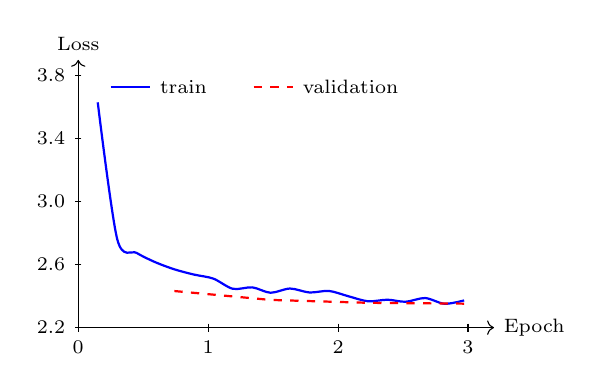
\begin{tikzpicture}[x=1.65cm,y=2.0cm,font=\scriptsize]
\draw[->] (0,0) -- (3.2,0) node[right] {Epoch};
\draw[->] (0,0) -- (0,1.7) node[above] {Loss};
\foreach \x in {0,1,2,3} {
    \draw (\x,0.025) -- (\x,-0.025) node[below] {\x};
}
\foreach \y/\lab in {0/2.2,0.4/2.6,0.8/3.0,1.2/3.4,1.6/3.8} {
    \draw (0.025,\y) -- (-0.025,\y) node[left] {\lab};
}
\draw[blue,thick] plot[smooth] coordinates {
    (0.15,1.4305) (0.30,0.5617) (0.45,0.4742) (0.59,0.4165)
    (0.74,0.3702) (0.89,0.3370) (1.04,0.3112) (1.19,0.2466)
    (1.34,0.2557) (1.48,0.2215) (1.63,0.2482) (1.78,0.2232)
    (1.93,0.2329) (2.08,0.1991) (2.23,0.1673) (2.38,0.1772)
    (2.52,0.1643) (2.67,0.1879) (2.82,0.1513) (2.97,0.1727)
};
\draw[red,dashed,thick] plot coordinates {
    (0.74,0.2323) (1.48,0.1759) (2.23,0.1576) (2.97,0.1522)
};
\draw[blue,thick] (0.25,1.53) -- (0.55,1.53) node[right,black] {train};
\draw[red,dashed,thick] (1.35,1.53) -- (1.65,1.53) node[right,black] {validation};
\end{tikzpicture}
\caption{Logged training and validation loss during full ViT5-base fine-tuning. The plotted vertical coordinates are shifted by 2.2 only for compact visualization; tick labels show the original loss values.}
\label{fig:loss_pretrained}
\end{figure}

\subsection{Qualitative Results}
Table~\ref{tab:qualitative} presents available examples generated by the scratch Transformer. These examples show that the scratch model often captures the broad topic but may omit names and numbers or introduce unrelated details.

\begin{table*}[htbp]
\centering
\caption{Qualitative examples available in the exported notebook snapshots.}
\label{tab:qualitative}
\begin{tabular}{p{0.31\textwidth}p{0.31\textwidth}p{0.31\textwidth}}
\toprule
Input document & Reference summary & Transformer from scratch \\
\midrule
MayTrip khai trương văn phòng mới tại 833 Lê Hồng Phong, TP HCM, giới thiệu nhiều ưu đãi du lịch và tour Hokkaido dịp Tết. & MayTrip mở văn phòng mới tại TP HCM để mở rộng dịch vụ phía Nam, đồng thời ra mắt nhiều voucher và tour Hokkaido. & Văn bản trên mô tả về sự kiện du lịch tại TP HCM. Các khách hàng có nhiều ưu đãi như du khách, du lịch và có thể tham quan các hoạt động du lịch. \\
\midrule
Đầu tháng 11, hoa dã quỳ nở tại Vườn quốc gia Ba Vì, tạo các vệt hoa vàng dọc đường mòn đi bộ dài hơn 3 km. & Rừng hoa dã quỳ ở Ba Vì rộng khoảng 10 ha, nở vào đầu tháng 11 và là điểm đến cuối thu được nhiều du khách yêu thích. & Một nhóm du khách nổi tiếng tại TP HCM trở thành chuyến du lịch nổi tiếng, trong đó có nhiều địa điểm như hoa, bánh mì và cây xanh. \\
\midrule
Việt Nam được Condé Nast Traveler xếp hạng 15 trong danh sách các quốc gia tốt nhất thế giới năm 2024; Thái Lan xếp thứ ba và Nhật Bản đứng đầu. & Việt Nam đứng thứ 15 với 89 điểm, Thái Lan xếp thứ ba và Nhật Bản đứng đầu bảng xếp hạng dựa trên đánh giá của độc giả Condé Nast Traveler. & Việt Nam là một trong những điểm du lịch nổi tiếng nhất thế giới. Sự kiện này bao gồm các trường du lịch, du lịch Việt Nam, Hàn Quốc, Nhật Bản và Thái Lan. \\
\bottomrule
\end{tabular}
\end{table*}

\begin{table*}[htbp]
\centering
\caption{Representative qualitative analysis of pre-trained-model validation predictions.}
\label{tab:qualitative_pretrained}
\begin{tabular}{p{0.13\textwidth}p{0.23\textwidth}p{0.37\textwidth}p{0.21\textwidth}}
\toprule
Model & Key source facts & Generated prediction & Analysis \\
\midrule
ViT5-base &
InterContinental Phu Quoc Long Beach Resort won a family-resort award in Asia for the second consecutive year and offers accommodation, wellness, entertainment, and dining services. &
Khu nghỉ dưỡng InterContinental Phu Quoc Long Beach Resort được vinh danh ở hạng mục gia đình trên toàn châu Á, nổi bật với thiết kế lấy cảm hứng từ đại dương. Khuôn viên rộng rãi với nhiều mảng xanh thiên nhiên đậm chất nhiệt đới. Du khách có thể chọn phòng khách sạn, căn hộ, suite hoặc biệt thự cao cấp hướng biển. Khu nghỉ dưỡng còn mang đến các liệu trình chăm sóc sức khỏe toàn diện. &
Fluent and faithful; preserves the main entity, award, design, accommodation, and wellness information. It omits the ``second consecutive year'' detail but introduces no clear unsupported fact. \\
\midrule
Qwen3-1.7B LoRA &
Japanese artist Miho Nakayama was found dead at her Tokyo home on December 6; the article reviews her acting and music career and her final social-media post. &
Nghệ sĩ Nhật Bản Miho Nakayama đã qua đời vào ngày 12/11, được tìm thấy trong nhà riêng của mình ở Tokyo. Cô đã có lịch sử thành công trong cả âm nhạc và phim trường, bao gồm cả các giải thưởng danh giá. Trước khi qua đời, cô đã đăng tải một trạng thái buồn bã trên mạng xã hội. &
Coherent and concise, but changes the date from December 6 to November 12. This is a clear numerical hallucination despite otherwise correct topic coverage. \\
\bottomrule
\end{tabular}
\end{table*}

The ViT5 example demonstrates the practical benefit of Vietnamese sequence-to-sequence pre-training: it compresses a long promotional article into a coherent summary while retaining multiple important aspects rather than merely naming the topic. The Qwen3 example remains fluent and captures the person's identity, career, location, and final social-media post, but its incorrect date illustrates that a high-level semantic match does not guarantee factual precision. Together with the aggregate metrics, these examples support selecting ViT5 as the final model and retaining explicit faithfulness instructions and entity/number checks for causal-LM variants. Aggregate output length also reveals a remaining control issue: ViT5 produces about 125 tokens on validation, close to its 160-token maximum.

% =========================================================
\section{Discussion and Error Analysis}

\subsection{Strengths and Weaknesses of the Transformer from Scratch}
The Transformer from scratch is designed to test whether the core attention-based encoder-decoder architecture can learn to generate summaries from the training data. Its main advantage is that all components are transparent and controllable, making it suitable for studying the internal mechanism of the Transformer. Since the implementation avoids \texttt{nn.Transformer}, each component can be inspected directly: attention projections, padding masks, causal masks, residual connections, Pre-LN normalization, and autoregressive decoding.

However, training from scratch requires substantial data and computation. Since the model starts from random initialization, it may learn slowly and produce less fluent summaries than a pre-trained model. In our experiments, the loss decreases steadily over 10 epochs and the repetition rate is nearly zero under no-repeat 3-gram blocking. The compression ratio is about 0.16 for beam decoding, showing that the model produces summaries that are substantially shorter than the input documents. Remaining qualitative issues should be analyzed manually from the generated JSONL outputs, especially missing fine-grained numerical details and possible hallucinated entities.

\subsection{Strengths and Weaknesses of the Pre-trained Model}
ViT5-base is substantially stronger than the scratch Transformer on every ROUGE metric. On the full test set, it improves ROUGE-1 by 0.1675, ROUGE-2 by 0.2637, and ROUGE-L by 0.1844. This supports the value of Vietnamese-specific pre-training: the model begins fine-tuning with useful lexical, syntactic, and semantic representations instead of learning language generation only from 10,775 training examples. The sampled resort prediction also shows strong multi-aspect coverage, retaining the named entity, award, design, accommodation options, and wellness services in a fluent paragraph.

The main cost is computational. Full ViT5 fine-tuning updates 227.72M parameters, compared with 11.47M for the scratch model. LoRA reduces the trainable ViT5 parameters to 1.77M, but its full-test ROUGE-L falls from 0.4889 to 0.4663. BARTpho is competitive at 0.4807 ROUGE-L, while the VietNews warm start reaches only 0.4728, showing that a task-specific warm start does not automatically transfer best to this dataset. The Qwen3 branch is flexible and supports explicit faithfulness instructions, but it is slower to generate, remains below ViT5 in the controlled subset experiments, and can alter critical numerical details such as dates.

\subsection{Error Categories}
We group common errors into the following categories:
\begin{itemize}
    \item \textbf{Missing key information}: the generated summary omits important entities, events, or numerical details.
    \item \textbf{Repetition}: the model repeats words, phrases, or clauses.
    \item \textbf{Hallucination}: the model generates information that is not supported by the source document.
    \item \textbf{Overly generic summary}: the output is fluent but too vague to represent the input document.
    \item \textbf{Length control problem}: the generated summary is too short or too long compared with the reference.
\end{itemize}

\begin{table*}[htbp]
\centering
\caption{Evidence-based error analysis from the exported experiment results.}
\label{tab:error_analysis}
\begin{tabular}{lp{0.38\textwidth}p{0.38\textwidth}}
\toprule
Error type & Scratch Transformer & Pre-trained model \\
\midrule
Missing key information & Observed; generated summaries often miss specific names, numbers, and locations. & ViT5 preserves several main aspects in the resort example but omits the ``second consecutive year'' detail. \\
Repetition & Low; Rep-3 is 0.0 with no-repeat 3-gram blocking. & No-repeat 3-gram blocking is enabled, but Rep-3 was not exported for pre-trained runs. \\
Hallucination & Observed in sampled outputs, especially incorrect locations or event details. & Qwen3 changes Miho Nakayama's reported date from December 6 to November 12; no clear hallucination is found in the sampled ViT5 output. \\
Too generic & Observed; some summaries overuse broad tourism/event phrases. & The sampled ViT5 and Qwen3 outputs are topic-specific and preserve the central named entity. \\
Length problem & Partly controlled; compression ratio is about 0.16 with beam decoding. & ViT5 averages 125 generated tokens on validation, while 15.05\% of references exceed 128 words. \\
\bottomrule
\end{tabular}
\end{table*}

\subsection{Why Causal Language Models Underperform}
The lower causal-LM scores should be interpreted as the combined effect of architecture, data characteristics, and experiment budget rather than as an intrinsic inability of causal models to summarize.

First, the dataset strongly favors source-grounded conditional generation. Validation references reuse 92.51\% of their unigrams and 68.99\% of their bigrams from the article. An encoder-decoder model separately encodes the complete source and generates the target through cross-attention, which is well suited to selecting and reorganizing source phrases. In contrast, a causal LM represents the instruction, article, and generated summary in one autoregressive stream. It may produce fluent paraphrases that are semantically reasonable but receive lower lexical-overlap ROUGE scores.

Second, encoder-decoder and causal models use their context budgets differently. ViT5 reserves up to 768 tokens for the encoder input and a separate 160-token decoder budget. The causal pipeline must include the instruction and article in its prompt before generating the summary. Prompt tokens and Vietnamese subword fragmentation reduce the effective article coverage. This explains why increasing Qwen3 source context from 768 to 1024 tokens raises validation-subset ROUGE-L from 0.3333 to 0.3792. The lead-coverage analysis also shows that the first quarter of an article contains only 51.31\% of validation-summary unigrams, so truncating later content can remove relevant facts.

Third, the target-length setting disadvantages the shorter causal runs. Validation summaries average 103.3 words, and 15.05\% contain more than 128 words. The main Qwen3 ablations limit targets to 128 subword tokens, so these long references, and likely additional references because of subword fragmentation, face substantial truncation pressure. ViT5 uses a larger 160-token target budget, providing 25\% more generation capacity. Only 0.30\% of validation references exceed 160 words, although token-level truncation may still affect a larger fraction.

Fourth, the training budgets are unequal. Full ViT5 fine-tuning uses all 10,775 training examples for three epochs, while controlled causal ablations use 2,500 or 7,000 examples and only 300 or 700 optimization steps. Their lower scores measure both model-family differences and limited adaptation. Finally, the dataset demands numerical faithfulness: 96.93\% of numbers in validation references are present in the source. The sampled Qwen3 date error demonstrates that an instruction-tuned causal LM can generate a plausible but unsupported number, which is strongly penalized by both ROUGE and human evaluation.

\subsection{Comparison Between Methods}
The completed experiments show a clear quality advantage for pre-trained sequence-to-sequence models. Full ViT5 fine-tuning improves full-validation ROUGE-L from 0.3053 to 0.4924 and full-test ROUGE-L from 0.3045 to 0.4889. It also more than doubles ROUGE-2 on the test set, indicating much stronger phrase-level content preservation. BARTpho approaches ViT5 but remains 0.0082 ROUGE-L lower on the full test set.

The scratch Transformer remains valuable because every architectural component is transparent and controllable, and its 11.47M parameters make it much smaller than ViT5. Its beam search slightly improves ROUGE-1 and ROUGE-2 over greedy decoding while maintaining zero repeated 3-grams. ViT5 LoRA offers the lowest adaptation cost, training only 0.777\% of the model, but loses 0.0190 validation ROUGE-L and 0.0226 test ROUGE-L relative to full fine-tuning.

The causal-LM experiments reveal that architecture alone is not enough. For Qwen3, extending the source context to 1024 tokens raises validation-subset ROUGE-L from 0.3333 to 0.3792 under otherwise similar rank-8 settings. Increasing rank and training data raises ROUGE-1 and ROUGE-2, but does not further improve ROUGE-L. Thus, source coverage is the most effective causal-LM improvement observed in our controlled ablations. However, the sampled date error shows that future causal-LM improvements should explicitly verify names, numbers, and dates rather than optimizing lexical overlap alone.

% =========================================================
\section{Conclusion}
In this project, we developed Vietnamese abstractive summarization systems using the two required approaches: a Transformer implemented and trained from scratch, and fine-tuned pre-trained language models below 3 billion parameters. The scratch Transformer implements the encoder-decoder architecture and practical training improvements directly. The primary pre-trained system fully fine-tunes ViT5-base, while additional experiments study ViT5 LoRA, BARTpho, a VietNews warm start, Qwen3, DeepSeek-R1-Distill-Qwen, prompt design, context length, and decoding.

The scratch Transformer reaches ROUGE-1/2/L of 0.5747/0.2038/0.3045 on the full test set. Full ViT5 fine-tuning achieves 0.7422/0.4675/0.4889 and is the strongest completed system. Its representative prediction is fluent, faithful, and covers several important aspects of a long article. LoRA greatly reduces the number of trainable parameters but introduces a measurable quality loss, and Qwen3 ablations show that longer source context is more beneficial than prompt tightening alone. Future work should broaden the human faithfulness audit and evaluate factuality with entity-, number-, and date-aware metrics in addition to ROUGE.

\section*{Code Availability}
The pre-trained-model training, LoRA, evaluation, final test comparison, and Kaggle experiment code is available at \url{https://github.com/Anhnguyen0812/pretrained-summarization}. The repository containing the Transformer-from-scratch implementation will be added separately. The reproducible train/validation-only dataset analysis is implemented in \texttt{analyze\_train\_valid\_dataset.py}; its output records the statistics reported in Tables~\ref{tab:dataset} and~\ref{tab:dataset_overlap}.

% =========================================================
\begin{thebibliography}{00}
\bibitem{vaswani2017attention}
A. Vaswani, N. Shazeer, N. Parmar, J. Uszkoreit, L. Jones, A. N. Gomez, L. Kaiser, and I. Polosukhin, ``Attention is All You Need,'' in \textit{Advances in Neural Information Processing Systems}, 2017.

\bibitem{lin2004rouge}
C.-Y. Lin, ``ROUGE: A Package for Automatic Evaluation of Summaries,'' in \textit{Proceedings of the ACL Workshop on Text Summarization Branches Out}, 2004.

\bibitem{lewis2020bart}
M. Lewis, Y. Liu, N. Goyal, M. Ghazvininejad, A. Mohamed, O. Levy, V. Stoyanov, and L. Zettlemoyer, ``BART: Denoising Sequence-to-Sequence Pre-training for Natural Language Generation, Translation, and Comprehension,'' in \textit{Proceedings of ACL}, 2020.

\bibitem{raffel2020t5}
C. Raffel, N. Shazeer, A. Roberts, K. Lee, S. Narang, M. Matena, Y. Zhou, W. Li, and P. J. Liu, ``Exploring the Limits of Transfer Learning with a Unified Text-to-Text Transformer,'' \textit{Journal of Machine Learning Research}, vol. 21, no. 140, pp. 1--67, 2020.

\bibitem{zhang2020pegasus}
J. Zhang, Y. Zhao, M. Saleh, and P. Liu, ``PEGASUS: Pre-training with Extracted Gap-sentences for Abstractive Summarization,'' in \textit{Proceedings of ICML}, 2020.

\bibitem{phan2022vit5}
L. Phan, H. Tran, H. Nguyen, and T. H. Trinh, ``ViT5: Pretrained Text-to-Text Transformer for Vietnamese Language Generation,'' in \textit{Proceedings of the 2022 Conference of the North American Chapter of the Association for Computational Linguistics: Student Research Workshop}, 2022.

\bibitem{tran2022bartpho}
N. L. Tran, D. M. Le, and D. Q. Nguyen, ``BARTpho: Pre-trained Sequence-to-Sequence Models for Vietnamese,'' in \textit{Proceedings of Interspeech}, 2022.

\bibitem{hu2022lora}
E. J. Hu, Y. Shen, P. Wallis, Z. Allen-Zhu, Y. Li, S. Wang, L. Wang, and W. Chen, ``LoRA: Low-Rank Adaptation of Large Language Models,'' in \textit{Proceedings of ICLR}, 2022.

\bibitem{yang2025qwen3}
A. Yang et al., ``Qwen3 Technical Report,'' arXiv preprint arXiv:2505.09388, 2025.
\end{thebibliography}

\balance
\end{document}
